\documentclass[tikz,border=1pt,convert=pdf2svg]{standalone}
\usepackage{laser_cut}

\newcommand\motorradius{1.46in/2}
\newcommand\spacing{\ledradius+0.5mm}
\newcommand\drawpair[2]{
	\draw (#1:#2)++(#1+90:\spacing) circle (\ledradius);
	\draw (#1:#2)++(#1-90:\spacing) circle (\ledradius);
}

\begin{document}
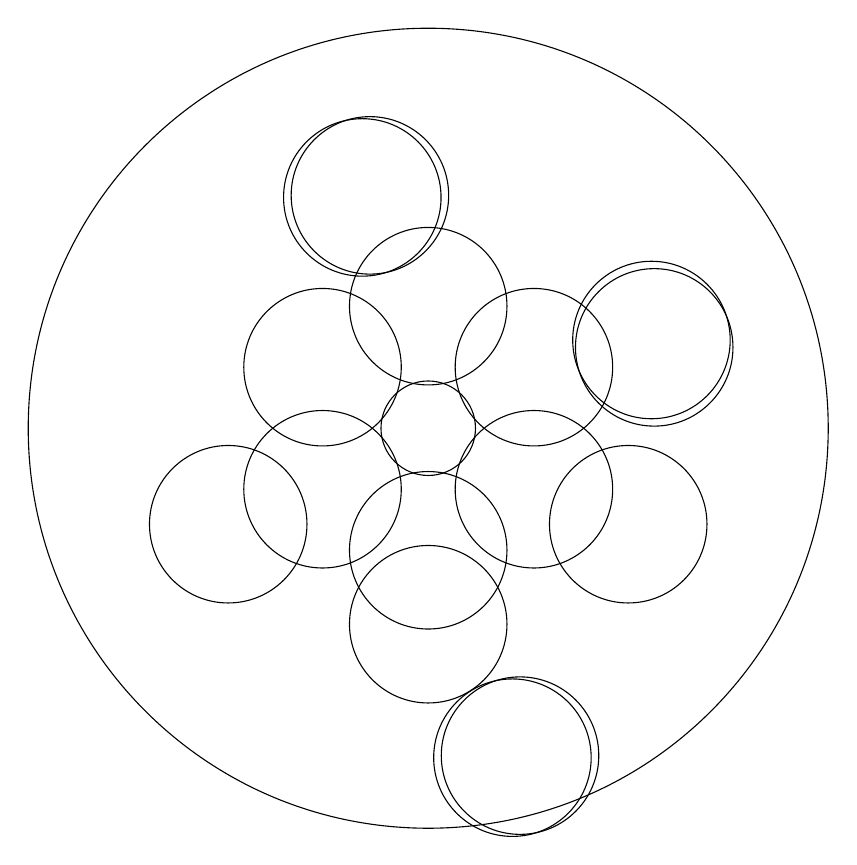
\begin{tikzpicture}
	\node (origin) at (0,0) {};
	\draw (origin) circle (4in/2); % size
	\draw (origin) circle (12mm/2); % center
	\draw (1in,-\motorradius+0.25in) circle (\sixthirtytworadius); % right frame hole
	\draw (-1in,-\motorradius+0.25in) circle (\sixthirtytworadius); % left frame hole
	\draw (0,-\motorradius-0.25in) circle (\sixthirtytworadius); % bottom frame hole
	\foreach \theta in {30,90,...,330} {
		\draw (origin)++(\theta:31mm/2) circle (\mthreefiveradius);
	}
	\drawpair{15+90}{1.2in}
	\drawpair{15+360/64}{1.2in}
	\drawpair{15-90}{1.7in}
\end{tikzpicture}
\end{document}


